\RequirePackage[T1]{fontenc}
\documentclass[conference,a4paper]{IEEEtran}
\usepackage[spanish,es-nodecimaldot]{babel}
\usepackage{amsmath,graphicx,booktabs,cite,microtype,listings}
\usepackage[hidelinks,breaklinks]{hyperref}
% Generado desde CSV/JSON: no editar a mano.
\newcommand{\Autor}{Angel Ramiro Apolo Aguilar}
\newcommand{\Correo}{angel.apolo@ucuenca.edu.ec}
\newcommand{\Universidad}{Universidad de Cuenca}
\newcommand{\Carrera}{Ingeniería en Telecomunicaciones}
\newcommand{\Asignatura}{Redes Vehiculares y Heterogéneas}
\newcommand{\Ciclo}{10.\textordmasculine{} ciclo}
\newcommand{\Accidentes}{16}
\newcommand{\Cerrados}{16}
\newcommand{\Mediana}{355,5}
\newcommand{\Pnoventa}{590,5}
\newcommand{\Media}{359,1}
\newcommand{\Maximo}{648,0}
\newcommand{\MedianaMision}{769,0}
\newcommand{\Migracion}{62,5}
\newcommand{\Flota}{10}
\newcommand{\Demanda}{4709}
\newcommand{\ColisionesBase}{9}
\newcommand{\DuracionBase}{449,08}
\newcommand{\GeoMax}{158,08}
\newcommand{\Controles}{649}
\newcommand{\Advertencias}{17}
\newcommand{\Repetidos}{7}
\newcommand{\FondoRetirado}{34}
\newcommand{\Negativas}{9}
\newcommand{\Planeados}{15}
\newcommand{\Naturales}{1}
\newcommand{\EstresAcc}{46}
\newcommand{\EstresCerr}{46}
\newcommand{\EstresMed}{328,5}
\newcommand{\EstresP}{670,5}
\newcommand{\MediaCercano}{268,3}
\newcommand{\MediaOrigen}{277,3}
\newcommand{\Diferencia}{9,0}
\newcommand{\Desviacion}{26,0}
\newcommand{\ParesGana}{4}
\newcommand{\EjemploAcc}{ACC04}
\newcommand{\EjemploHospital}{Militar}
\newcommand{\EjemploRango}{6}
\newcommand{\UsoHospital}{Vicente Corral}
\newcommand{\UsoPublico}{14,2}
\newcommand{\GuiAcc}{ACC05}
\newcommand{\GuiTiempo}{2611}
\newcommand{\GuiUnidad}{U02}
\newcommand{\GuiOrigen}{Vicente Corral}
\newcommand{\GuiDestino}{M. Patamarca}
\newcommand{\GuiAntes}{3}
\newcommand{\GuiDespues}{4}
\newcommand{\GuiRetorno}{2776}

\hypersetup{pdftitle={Práctica 04: accidentes bus-moto y despacho de ambulancias},pdfauthor={Angel Ramiro Apolo Aguilar}}
\graphicspath{{figuras/}{capturas/}{../../salida/figuras/}{../../salida/visual/}}
\addto\captionsspanish{\renewcommand{\tablename}{Tabla}\renewcommand{\abstractname}{Resumen}}
\renewcommand{\IEEEkeywordsname}{Palabras clave}
\lstset{basicstyle=\ttfamily\footnotesize,breaklines=true,columns=fullflexible,keepspaces=true,showstringspaces=false,frame=single,framerule=0.2pt}
\newcommand{\archivo}[1]{\texttt{\detokenize{#1}}}
\begin{document}
\title{Accidentes bus-moto y despacho de ambulancias en Cuenca mediante SUMO y TraCI}
\author{\IEEEauthorblockN{\Autor}
\IEEEauthorblockA{\Carrera, \Ciclo\\\Universidad, Cuenca, Ecuador\\
\Asignatura\\\Correo}}
\maketitle

\begin{abstract}
Esta práctica estudia cómo los accidentes entre buses y motocicletas afectan el despacho y la disponibilidad de ambulancias en una red de Cuenca. El escenario se ejecutó con un simulador de tráfico microscópico y un controlador en Python que detecta colisiones, asigna unidades hospitalarias y sigue cada misión hasta su retorno. La red docente recortada contiene 1.745 aristas y 176 semáforos. La línea base incorporó \Demanda{} vehículos durante tres horas de demanda. En la corrida principal se atendieron \Accidentes{} accidentes y se cerraron todas las misiones, con una mediana de respuesta de \Mediana{} segundos y un percentil 90 de \Pnoventa{} segundos. La flota conservó sus diez unidades y no se registraron teletransportaciones. La repetición produjo siete archivos idénticos. También se compararon dos políticas de retorno con cinco semillas y una carga de quince accidentes por hora. La validación espacial permanece parcial: el punto de Patamarca está a \GeoMax{} metros del acceso vial asignado, por encima del límite de 150 metros.
\end{abstract}
\begin{IEEEkeywords}
simulación de tráfico, despacho de ambulancias, colisiones, SUMO, TraCI.
\end{IEEEkeywords}

\section{Introducción}
Un accidente cambia las condiciones de circulación de la vía en la que ocurre. Si los vehículos permanecen detenidos, la ambulancia debe atravesar el tráfico que el propio incidente genera. La respuesta depende de la ruta disponible, del número de unidades en cada hospital y de las decisiones tomadas después de atender casos anteriores.

La Práctica 04 de Redes Vehiculares y Heterogéneas plantea este problema sobre una red de Cuenca\cite{guia}. El trabajo desarrolla las fases F0 a F5: preparación vial, demanda de fondo, ubicación de hospitales, generación de choques, despacho y análisis. El objetivo es comprobar que cada incidente tenga una colisión física como evidencia y que las ambulancias conserven su identidad durante toda la misión. La comparación entre retorno al origen y retorno al hospital más cercano permite observar cómo cambia la distribución de unidades disponibles.

El estudio corresponde al componente de tráfico y control de la asignatura. No incorpora comunicación inalámbrica ni estima tiempos reales de un servicio de emergencias. Los parámetros de demanda, flota y atención pertenecen al ejercicio académico.

\section{Escenario y metodología}
\subsection{Procedencia y reducción de la red}
El archivo \archivo{cuenca_net.xml} procede del ZIP docente aportado para la práctica. El original y su huella SHA-256 se conservan en \archivo{datos/docente/} y \archivo{datos/procedencia_red.json}. Sobre esta red se ejecuta una única llamada a \archivo{netconvert}, con el recorte geográfico de la guía: longitudes entre $-79{,}030$ y $-78{,}950$, y latitudes entre $-2{,}930$ y $-2{,}860$.

Se mantienen vías de categoría \archivo{tertiary} o superior y la mayor componente débil; se eliminan aristas aisladas y se simplifica la geometría. La opción \archivo{junctions.join-dist=25} agrupa cruces próximos dentro del umbral indicado. Los giros en U se permiten únicamente en terminales. El resultado coincide con los 1.745 aristas y 176 semáforos de la guía. La Tabla~\ref{tab:red} compara ambas redes; las longitudes suman aristas dirigidas, por lo que una calle de doble sentido puede contribuir dos veces.

\begin{table}[!t]
\caption{Red original y red de avenidas}
\label{tab:red}\centering\footnotesize
\begin{tabular}{lrrr}
\toprule
Red & Aristas & Semáforos & km dirigidos \\
\midrule
Completa & 34256 & 337 & 3984,3 \\
Recortada & 1745 & 176 & 355,6 \\
\bottomrule
\end{tabular}

\end{table}

\subsection{Demanda y configuración de ejecución}
La demanda dura 10.800 s y solicita 1.200 automóviles/h, 100 buses/h y 300 motocicletas/h. Las tres llamadas a \archivo{randomTrips.py} usan semilla 42 y validan las rutas. Después de descartar viajes sin conexión, circulan \Demanda{} vehículos de fondo. El horizonte total es de 12.600 s, con un paso de 1 s; los últimos 1.800 s permiten vaciar la red.

La simulación utiliza SUMO 1.12.0, disponible en la imagen \archivo{van3twin:jammy}. Las opciones \archivo{time-to-teleport=-1} y \archivo{time-to-teleport.disconnected=-1} impiden resolver bloqueos mediante teletransportación. La acción de colisión es \archivo{warn}; se revisan cruces y se usa \archivo{collision.mingap-factor=0} para exigir contacto físico. El 30\% de los vehículos actualiza su ruta cada 120 s. Las opciones y tipos de vehículo completos están en \archivo{escenario/}.

\subsection{Hospitales y conservación de unidades}
El ZIP docente contiene únicamente la red. Por ello, los siete puntos hospitalarios se obtienen del archivo OpenStreetMap conservado en el proyecto\cite{osm}. Los polígonos se representan por su centroide; El Valle es un nodo. Estas coordenadas identifican instalaciones y no equivalen a entradas de urgencias verificadas. La Fig.~\ref{fig:mapa} muestra su distribución y los incidentes de la corrida principal.

Cada punto se proyecta mediante \archivo{convertRoad} con clase \archivo{emergency}. Se comprueba el acceso de ida y vuelta respecto a Vicente Corral Moscoso. Cuando la proyección más próxima carece de retorno, se busca el carril permitido más cercano con ambas rutas. La tabla de resultados conserva tanto la proyección inicial como el acceso corregido. La conectividad dirigida se verifica para los 49 pares de hospitales.

Las unidades disponibles se guardan en colas FIFO. Con semilla 42, los cinco hospitales públicos reciben $[3,1,1,3,2]$ unidades y los dos privados $[0,0]$. Cada ambulancia tiene un identificador persistente; su vehículo en SUMO es la representación de una misión. En cada segundo se verifica
\begin{equation}
\sum_h N_h^{\text{disponible}}(t)+N^{\text{misión}}(t)=10.
\label{eq:flota}
\end{equation}
También se comprueba que ninguna identidad esté duplicada.

\begin{figure*}[!t]
\centering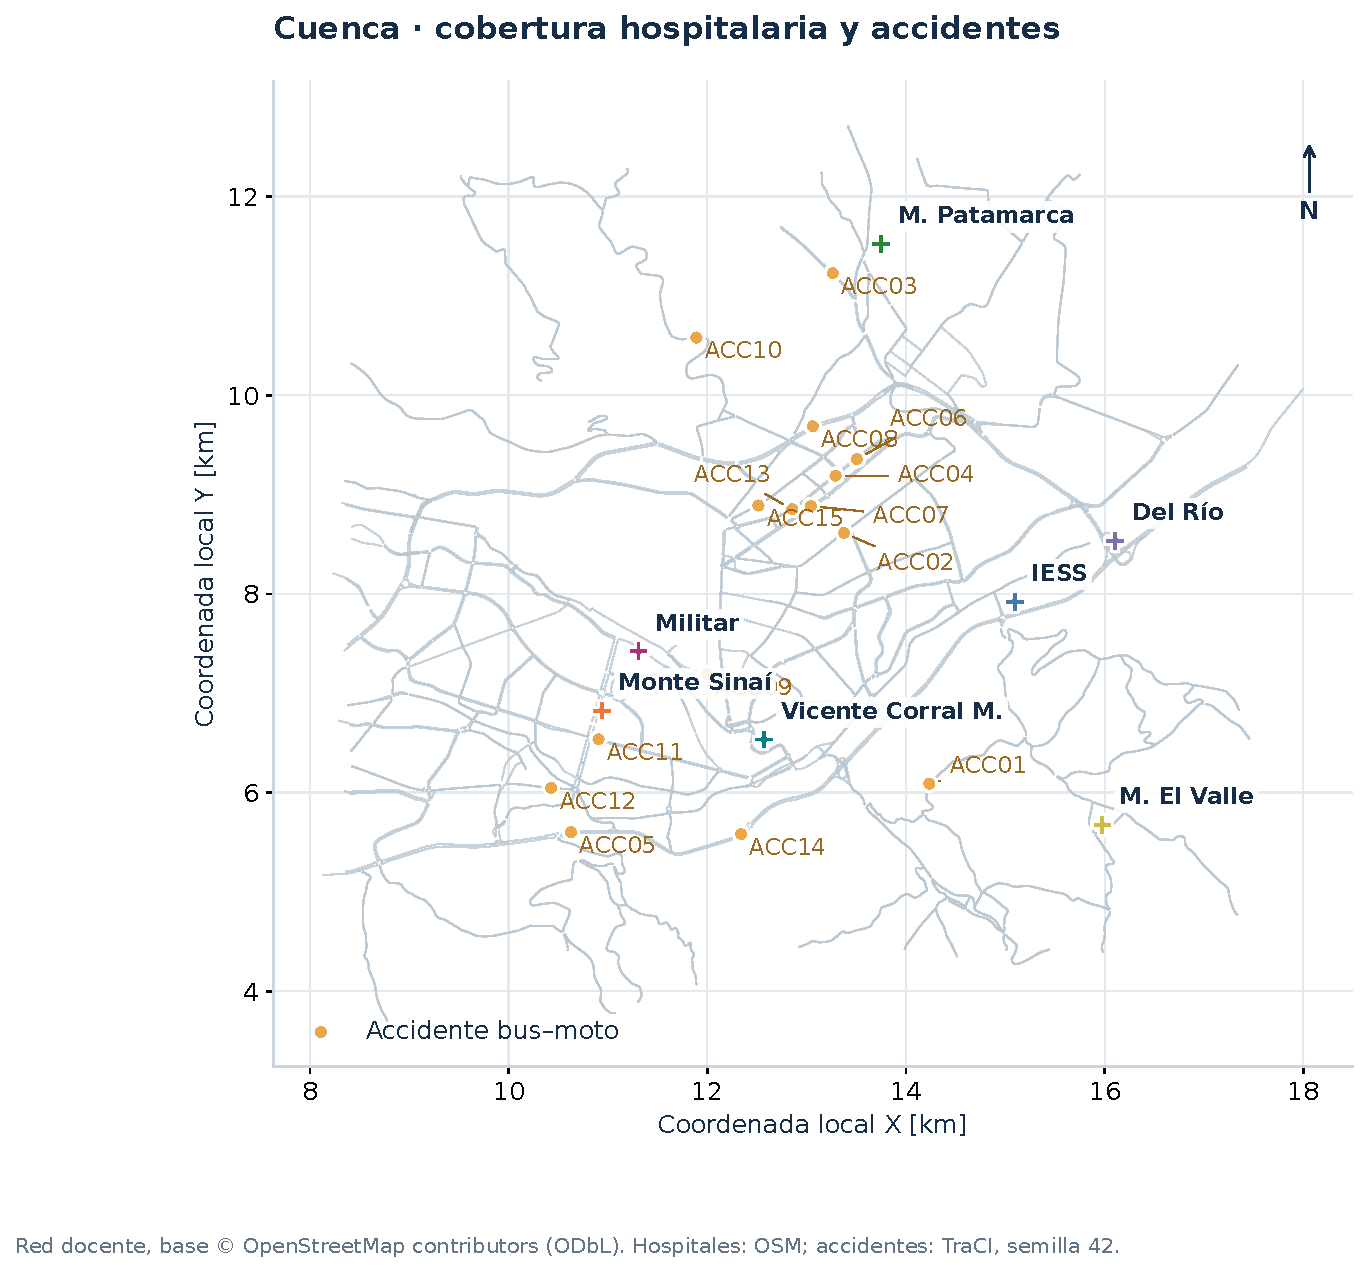
\includegraphics[width=0.83\textwidth]{01_mapa.pdf}
\caption{Red de estudio, hospitales y accidentes de la corrida principal. Las posiciones hospitalarias proceden de OpenStreetMap; los incidentes se registran mediante TraCI.}
\label{fig:mapa}
\end{figure*}

\subsection{Generación y detección de accidentes}
La agenda programa cinco intentos por hora entre los minutos 5 y 58. El controlador elige un bus que circule en una arista externa, haya avanzado más de 60 m y tenga una velocidad de al menos 4 m/s. La implementación limita la selección a 18 m/s y exige longitud suficiente para que el alcance ocurra antes del siguiente cruce. También verifica el acceso de ida y vuelta de la ambulancia. Esta selección restringe los lugares en los que pueden aparecer los incidentes programados.

La motocicleta se inserta 45 m detrás del bus, en su mismo carril y con el resto de su ruta. Cuando aparece en la simulación se aplican \archivo{setSpeedMode(0)}, \archivo{setLaneChangeMode(0)} y \archivo{setSpeed(22)}. El incidente solo se registra si SUMO informa una colisión física bus-moto; los intentos fallidos se reprograman y las parejas ya detectadas no vuelven a contarse. Si no hay un bus apto, se revisa de nuevo 20 s después. Un intento expira a los 90 s, o antes si la pareja abandona la arista o desaparece; en ese caso se reprograma 60 s después.

El bit 0 de \archivo{speedMode} controla la velocidad segura\cite{traci}. Pedir una velocidad alta con el modo 31 conserva esa restricción. La prueba en una recta aislada, resumida en la Tabla~\ref{tab:modos}, permite separar este efecto de las condiciones del mapa urbano. El modo 0 mantiene la interpretación heredada de SUMO, por lo que no debe describirse como la desactivación de todos los bits actuales.

\begin{table}[!t]
\caption{Prueba aislada del control de velocidad}
\label{tab:modos}\centering\footnotesize
\begin{tabular}{rc}
\toprule
Modo & Colisión \\
\midrule
31 & No \\
30 & Sí \\
23 & No \\
0 & Sí \\
\bottomrule
\end{tabular}

\end{table}

Tras detectar el choque, bus y moto quedan inmóviles y se colorean en rojo. Durante dos pasos se usa modo 0 para detenerlos; luego se restaura el modo 31 manteniendo velocidad cero. Las demás colisiones de fondo se registran y sus vehículos se retiran, salvo ambulancias y víctimas protegidas. En la corrida principal se retiraron \FondoRetirado{} vehículos por este motivo. Esta intervención forma parte del modelo y afecta al tráfico posterior.

\subsection{Despacho, llegada y retorno}
El controlador calcula rutas desde los hospitales con \archivo{findRoute} y modo de enrutamiento agregado, que usa tiempos de viaje suavizados\cite{routing}. Los candidatos se ordenan por tiempo estimado. Un hospital sin stock se descarta; si tiene unidades, puede negar disponibilidad con probabilidad $0{,}25$. Se toma la primera unidad de la cola del primer candidato aceptado. Si todos se descartan, el accidente espera y se revisa cada 30 s.

La llegada se reconoce por uno de estos criterios: distancia de conducción de hasta 50 m; ambulancia detenida detrás del accidente en la misma arista; o detención de al menos 30 s a una distancia euclídea de hasta 300 m. El tercer criterio representa una atención a pie aproximada, sin simular peatones ni sumar un tiempo de caminata. Cada incidente conserva el criterio utilizado.

La atención dura 120 s. Después se retiran los vehículos accidentados y la ambulancia regresa al hospital con menor tiempo de ruta desde la arista del incidente. En la política alternativa regresa al hospital de origen. El retorno restablece los controles:
\begin{lstlisting}[language=Python]
traci.vehicle.setSpeedMode(veh, 31)
traci.vehicle.setLaneChangeMode(veh, 1621)
traci.vehicle.setSpeed(veh, -1)
traci.vehicle.changeTarget(veh, hospital.edge)
\end{lstlisting}
La unidad se incorpora a la cola destino únicamente cuando se observa la llegada del vehículo. En SUMO 1.12, \archivo{arrivalPos=max} representa el extremo de la arista hospitalaria; este detalle limita la precisión espacial del retorno.

\subsection{Medidas y diseño de la comparación}
Los datos macroscópicos se recogen cada 900 s con \archivo{edgeData}\cite{macro}. Para cada arista $e$ e intervalo de duración $\Delta t$ se calcula
\begin{align}
q_e&=\mathrm{entered}_e\frac{3600}{\Delta t},\\
k_e&=\mathrm{density}_e,\qquad v_e=3{,}6\,\mathrm{speed}_e.
\end{align}
El flujo $q$ se expresa en veh/h, la densidad $k$ en veh/km de arista y la velocidad $v$ en km/h. Los valores de $q$ y $k$ se ponderan por longitud; $v$ se pondera por flujo. Se calcula por separado la media de $k_e v_e$, ya que el producto de medias con pesos diferentes no tiene por qué coincidir con ella. El régimen estacionario comprende de 900 a 10.800 s.

Para cada misión se distinguen espera $T_e$, desplazamiento $T_d$ y respuesta total $T_r$:
\begin{equation}
T_r=t_{\mathrm{llegada}}-t_{\mathrm{accidente}}=T_e+T_d.
\end{equation}
La duración de misión se mide desde el despacho hasta la disponibilidad en el hospital destino. La mediana y el percentil 90 se calculan sobre misiones cerradas; los casos abiertos se conservan como censurados. El percentil usa interpolación lineal.

Se comparan ambas políticas con semillas 8, 21, 42, 84 y 123. La demanda se mantiene fija y se separan los generadores aleatorios de flota, agenda, selección del bus y disponibilidad. Las corridas comparten semilla, pero las decisiones modifican el tráfico y pueden cambiar el lugar de los accidentes. Una corrida adicional aumenta la agenda a quince incidentes por hora.

\section{Resultados}
\subsection{Tráfico de fondo y control espacial}
La línea base insertó \Demanda{} vehículos y terminó sin activos ni teletransportaciones. Registró \ColisionesBase{} colisiones de fondo y una duración media de viaje de \DuracionBase{} s. La Fig.~\ref{fig:macro} muestra la evolución temporal y la Tabla~\ref{tab:avenidas} resume las tres avenidas solicitadas. La Fig.~\ref{fig:fundamental} relaciona flujo, densidad y velocidad. Los promedios de densidad por avenida son bajos, aunque no descartan colas locales. Con esta demanda no se estima una capacidad vial calibrada.

\begin{figure*}[!t]
\centering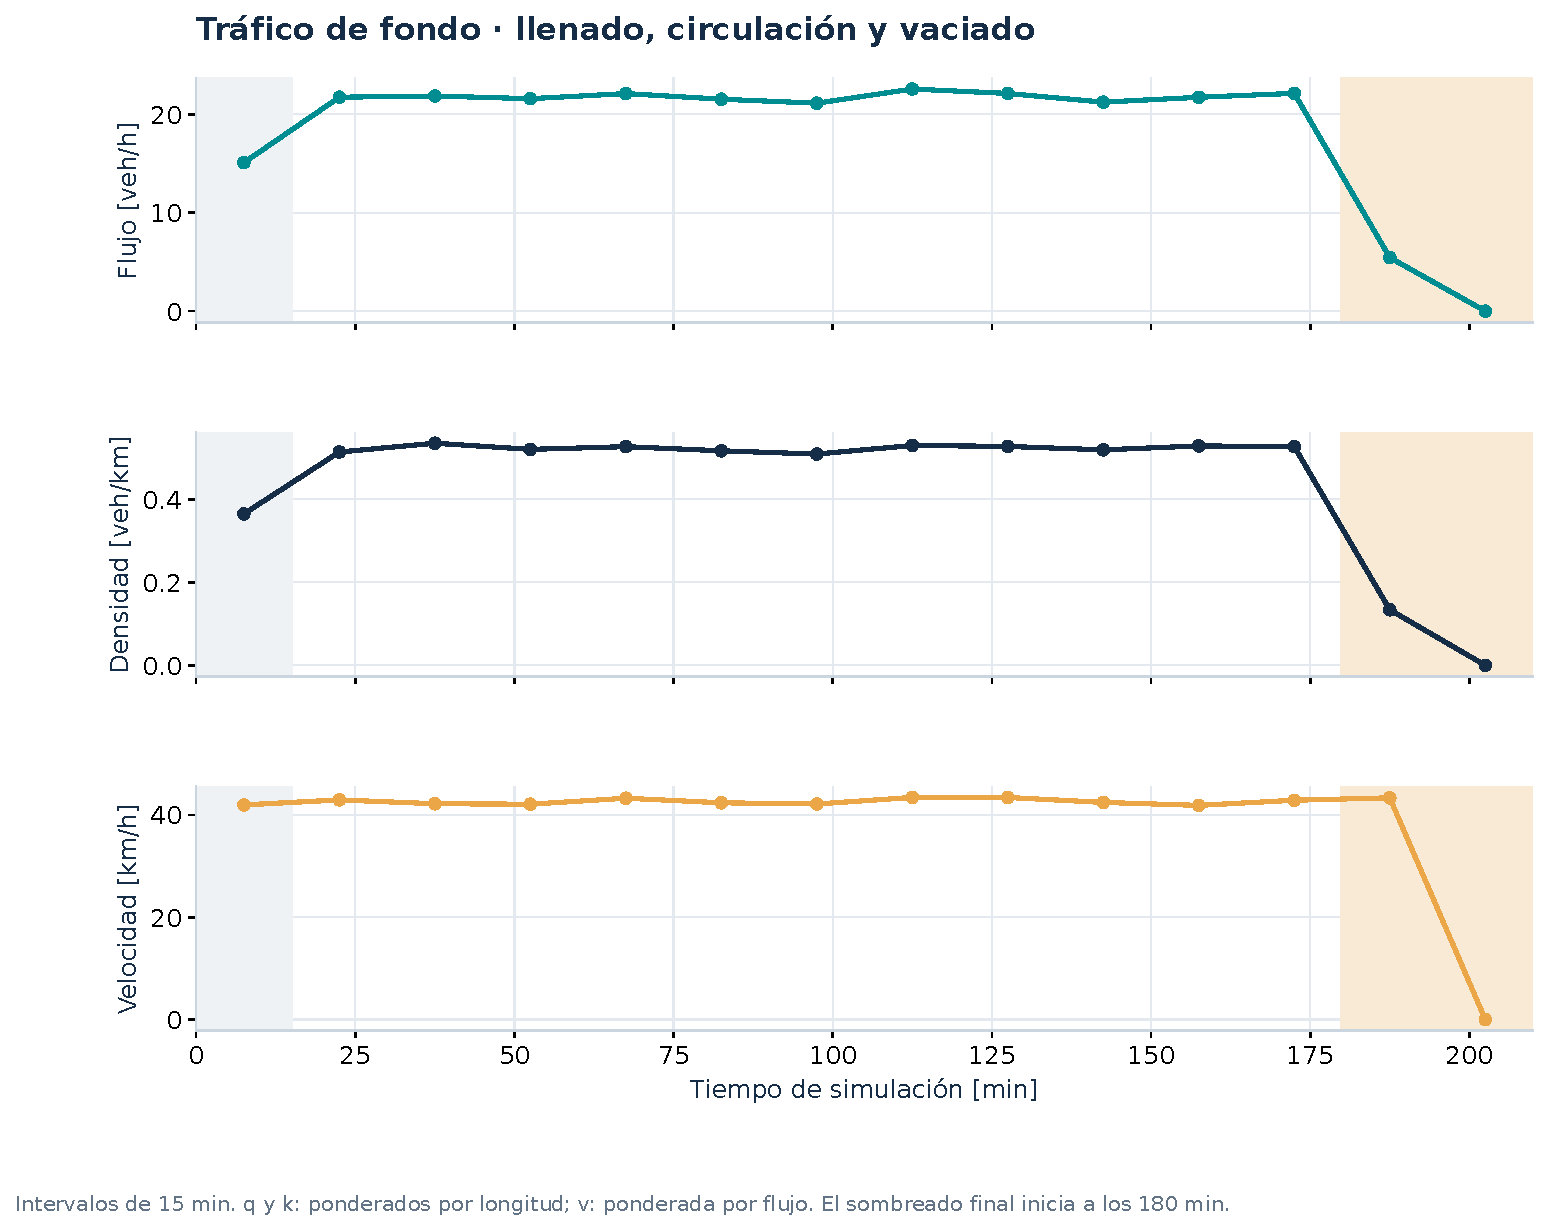
\includegraphics[width=0.95\textwidth]{02_trafico_macro.pdf}
\caption{Evolución macroscópica de la línea base. La demanda termina a los 180 min; la ejecución continúa hasta los 210 min para observar el vaciado.}
\label{fig:macro}
\end{figure*}

\begin{table*}[!t]
\caption{Avenidas durante el régimen estacionario}
\label{tab:avenidas}\centering\footnotesize
\begin{tabular}{lrrrrr}
\toprule
Avenida & $q$ [veh/h] & $k$ [veh/km] & $v$ [km/h] & $\overline{kv}$ [veh/h] & Error [\%] \\
\midrule
Huayna Cápac & 91,32 & 2,91 & 32,60 & 96,00 & -4,88 \\
Las Américas & 61,59 & 1,39 & 47,71 & 64,00 & -3,77 \\
Circunvalación Sur & 87,98 & 1,15 & 72,98 & 90,31 & -2,58 \\
\bottomrule
\end{tabular}

\end{table*}

\begin{figure*}[!t]
\centering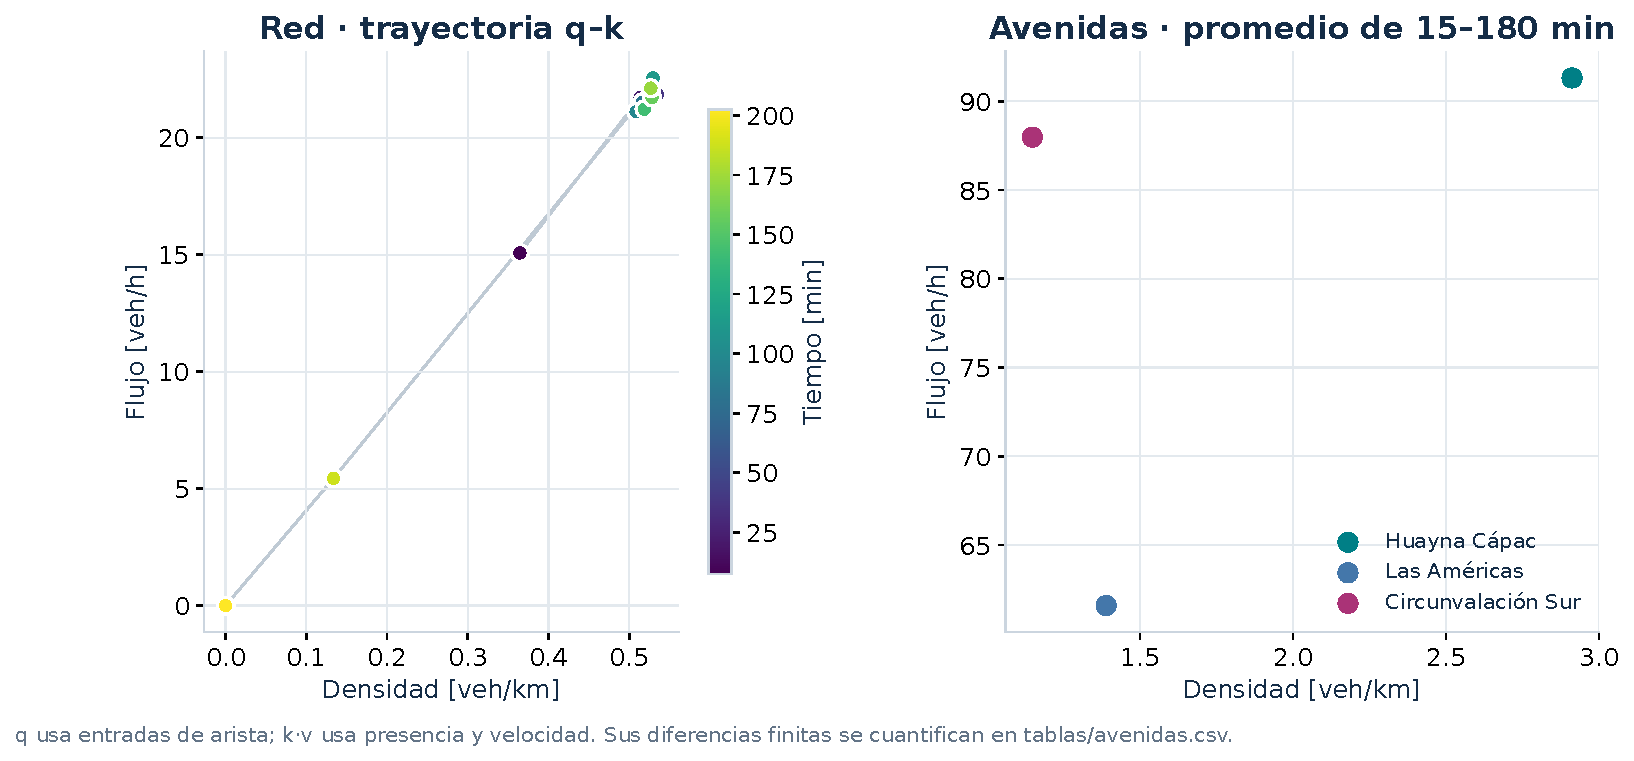
\includegraphics[width=0.95\textwidth]{03_diagrama_fundamental.pdf}
\caption{Relaciones entre flujo, densidad y velocidad. La diferencia entre el flujo por entradas y la media de $kv$ se conserva en las tablas.}
\label{fig:fundamental}
\end{figure*}

Los 49 pares hospitalarios tienen rutas dirigidas válidas para la clase de ambulancia. Seis puntos cumplen el límite espacial del taller. Patamarca queda a \GeoMax{} m del acceso asignado: el criterio A3 continúa parcial. Su coordenada representa el centroide del establecimiento y la vía local Del Camal se excluye al conservar avenidas. Corregir este punto requiere una entrada verificada o la coordenada del capítulo del estudiante.

\subsection{Respuesta y distribución de ambulancias}
La corrida principal produjo \Planeados{} incidentes de la agenda y \Naturales{} natural, para un total de \Accidentes. Todas las misiones cerraron. La mediana de respuesta fue \Mediana{} s y el percentil 90, \Pnoventa{} s; la media alcanzó \Media{} s y el máximo, \Maximo{} s. La espera de despacho fue cero, de modo que la respuesta total coincide con el desplazamiento en esta corrida. La mediana de misión completa fue \MedianaMision{} s.

La Fig.~\ref{fig:respuesta} permite comparar los incidentes sin ocultar los casos lentos. La selección por tiempo de ruta tampoco implica que siempre salga el primer hospital del ranking. Por ejemplo, \EjemploAcc{} fue atendido desde \EjemploHospital{}, que ocupaba el puesto \EjemploRango. La Tabla~\ref{tab:despacho} muestra los descartes previos registrados por el controlador.

\begin{figure*}[!t]
\centering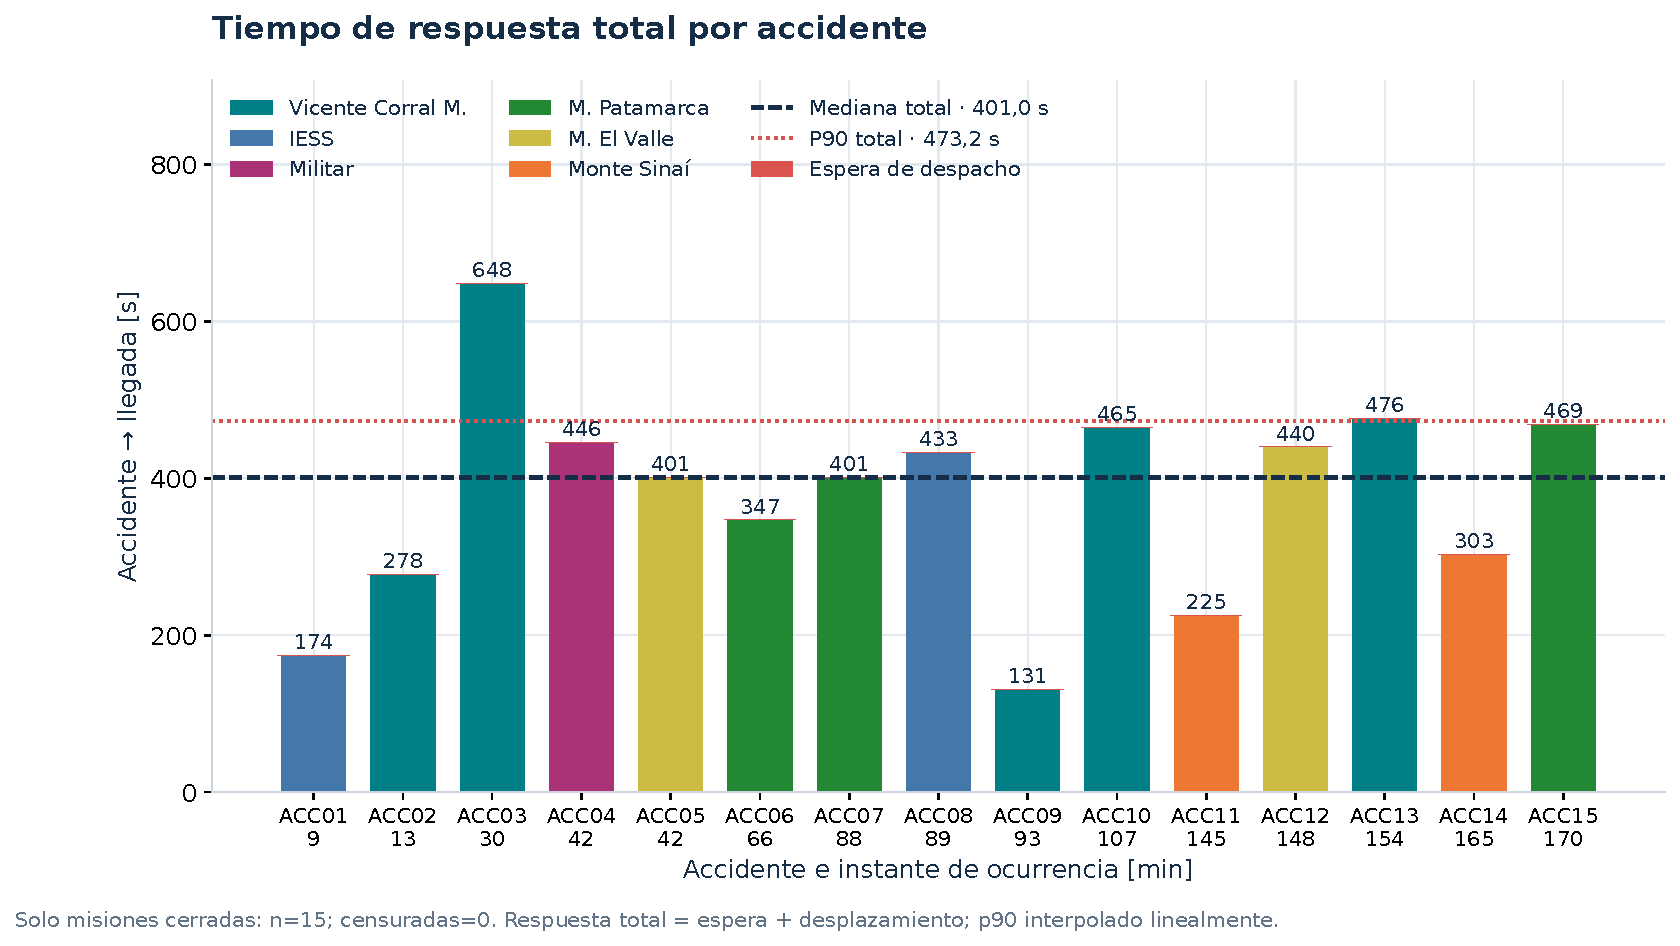
\includegraphics[width=0.97\textwidth]{04_respuesta.pdf}
\caption{Tiempo de respuesta por accidente y hospital de salida. Las líneas indican mediana y percentil 90; la espera de despacho es cero en la semilla principal.}
\label{fig:respuesta}
\end{figure*}

\begin{table*}[!t]
\caption{Candidatos de despacho para \EjemploAcc}
\label{tab:despacho}\centering\footnotesize
\begin{tabular}{rlrrl}
\toprule
Rango & Hospital & ETA [s] & Stock & Decisión \\
\midrule
1 & Del Río & 292,8 & 0 & Sin unidades \\
2 & Vicente Corral & 301,3 & 2 & Negativa \\
3 & M. Patamarca & 316,0 & 3 & Negativa \\
4 & IESS & 395,9 & 0 & Sin unidades \\
5 & Monte Sinaí & 396,1 & 0 & Sin unidades \\
6 & Militar & 437,6 & 1 & Despacho \\
\bottomrule
\end{tabular}

\end{table*}

La flota conservó \Flota{} unidades. El \Migracion\% de las misiones terminó en un hospital diferente del de salida. Patamarca pasó de tres a cinco unidades disponibles, mientras Monte Sinaí pasó de cero a tres. Este último pudo despachar después de recibir unidades. La Tabla~\ref{tab:hospitales} y las Figs.~\ref{fig:hospitales} y~\ref{fig:migracion} muestran el balance y su evolución temporal.

\begin{table*}[!t]
\caption{Acceso hospitalario, balance de flota e índice de utilización}
\label{tab:hospitales}\centering\footnotesize
\begin{tabular}{lrrrrrr}
\toprule
Hospital & Dist. [m] & Inicial & Final & Despachos & Recibidas & Uso [\%] \\
\midrule
Vicente Corral & 102,20 & 3 & 1 & 5 & 3 & 12,5 \\
IESS & 117,76 & 1 & 0 & 2 & 1 & 11,7 \\
Militar & 26,68 & 1 & 0 & 1 & 0 & 7,7 \\
M. Patamarca & 135,32 & 3 & 6 & 3 & 6 & 8,1 \\
M. El Valle & 54,81 & 2 & 1 & 2 & 1 & 7,2 \\
Monte Sinaí & 29,04 & 0 & 2 & 2 & 4 & N/A \\
Del Río & 88,65 & 0 & 0 & 0 & 0 & N/A \\
\bottomrule
\end{tabular}

\end{table*}

\begin{figure*}[!t]
\centering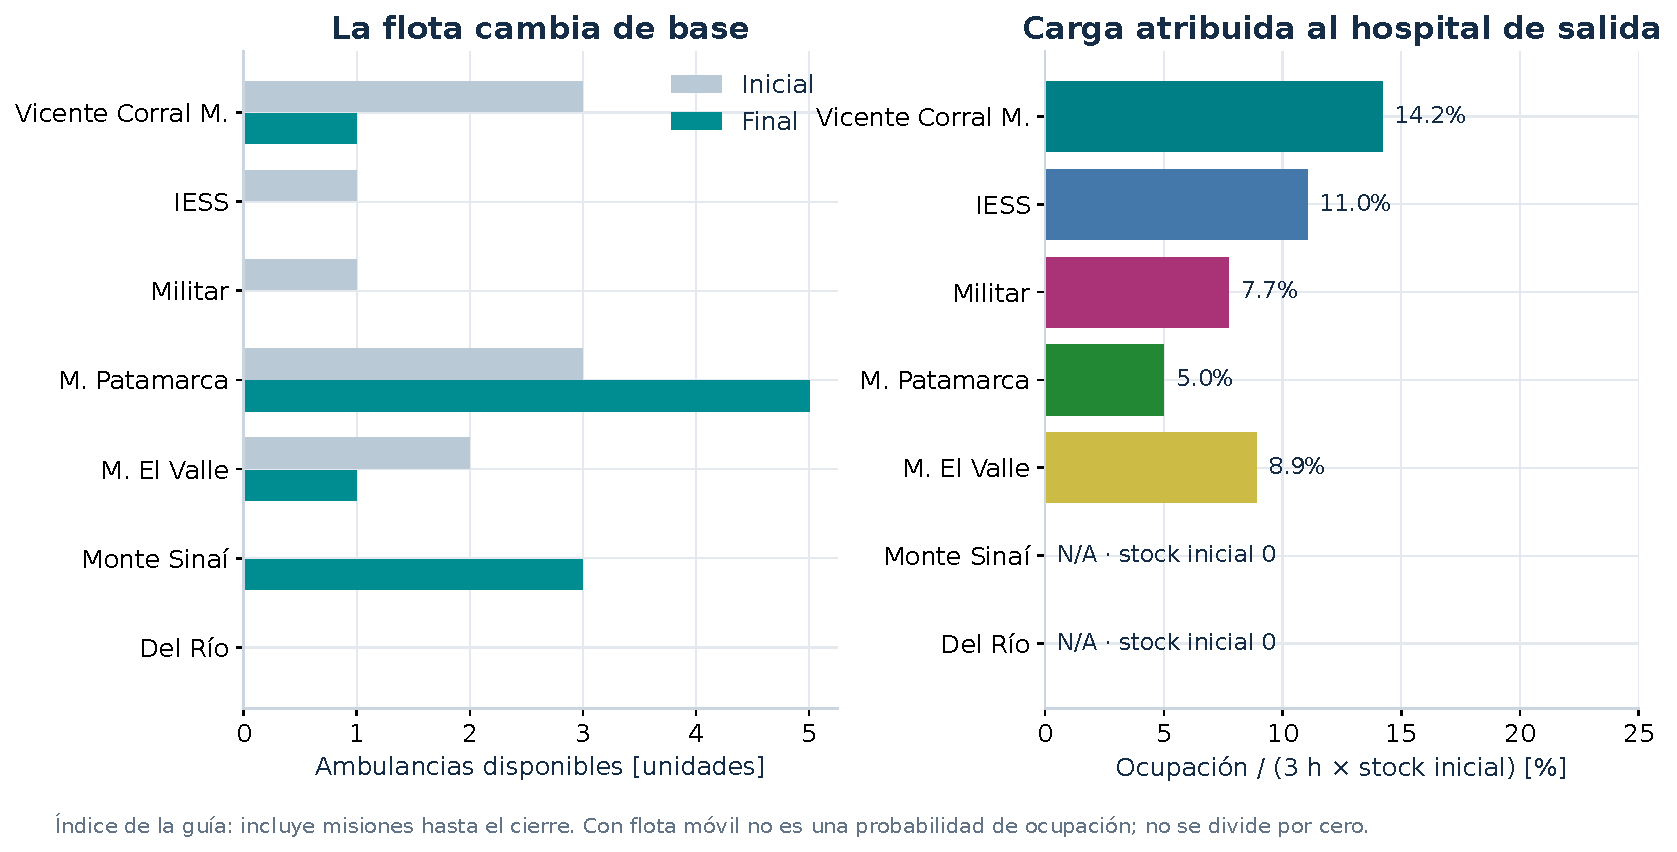
\includegraphics[width=0.95\textwidth]{05_hospitales.pdf}
\caption{Despachos e índice de utilización por hospital. N/A indica un denominador de stock inicial igual a cero.}
\label{fig:hospitales}
\end{figure*}

La utilización divide el tiempo ocupado atribuido al hospital de salida por $10.800$ s multiplicados por su stock inicial. Con una flota que cambia de base, este cociente es un índice de carga y no una probabilidad de ocupación de unidades fijas. \UsoHospital{} presentó el mayor índice público, con \UsoPublico\%. Los hospitales con stock inicial cero se informan como N/A.

\begin{figure*}[!t]
\centering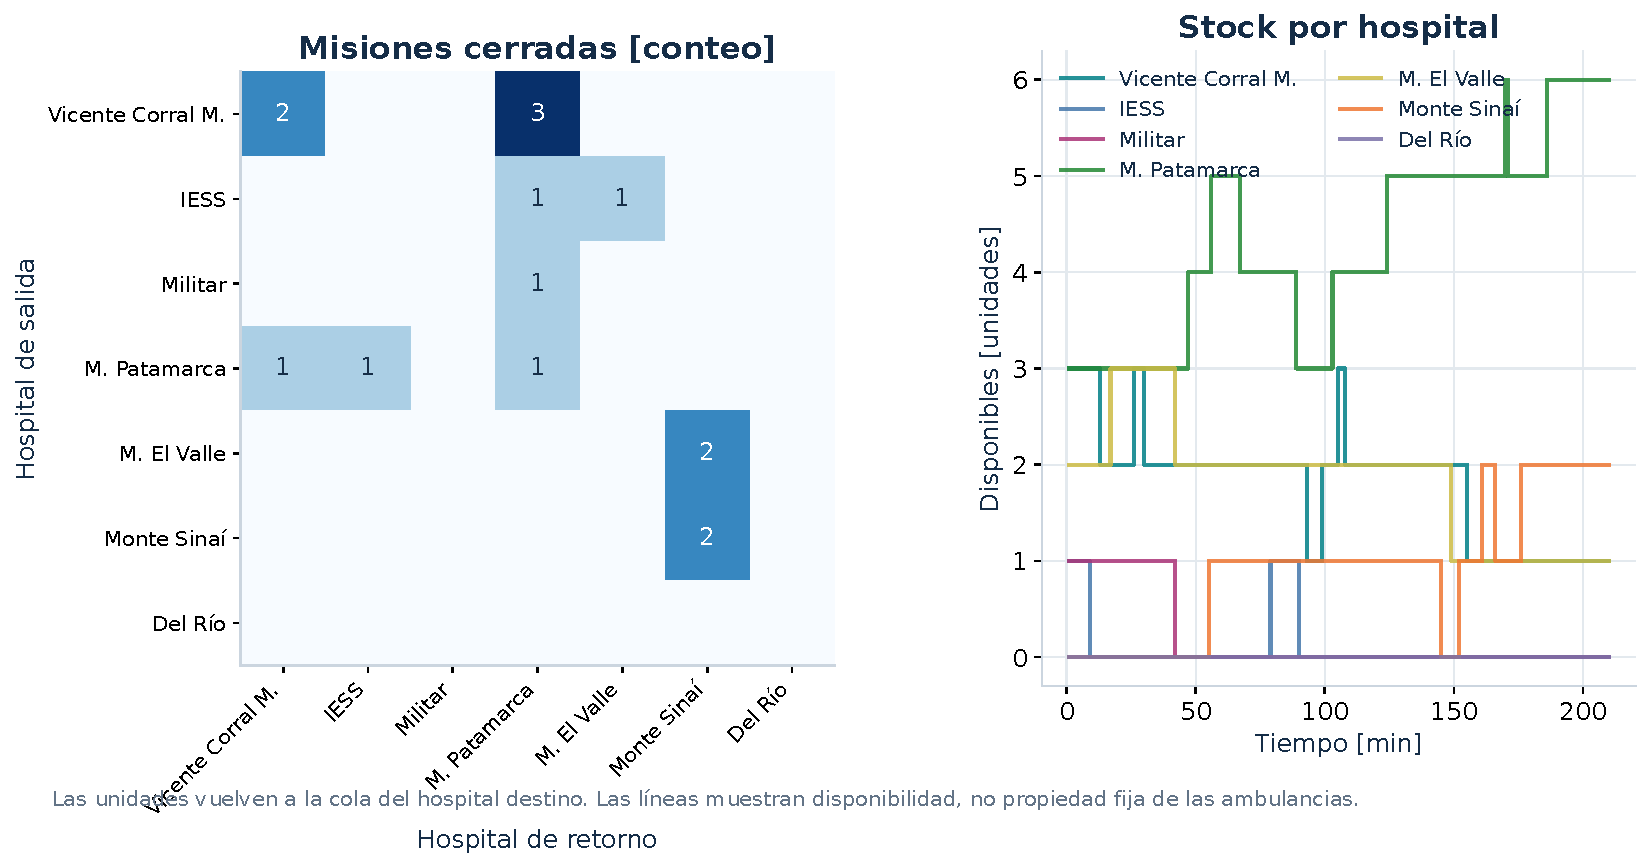
\includegraphics[width=0.95\textwidth]{06_migracion.pdf}
\caption{Matriz de retorno y disponibilidad hospitalaria. Cada unidad se suma al destino cuando termina su misión.}
\label{fig:migracion}
\end{figure*}

\subsection{Políticas de retorno y aumento de carga}
La media de las medianas fue \MediaCercano{} s para retorno cercano y \MediaOrigen{} s para retorno al origen. La diferencia origen menos cercano promedió \Diferencia{} s, con desviación muestral de \Desviacion{} s. El retorno cercano obtuvo menor mediana en \ParesGana{} de los cinco pares (Tabla~\ref{tab:politicas}). La variación de la Fig.~\ref{fig:extension} aconseja limitar la conclusión a estas corridas.

\begin{table*}[!t]
\caption{Comparación por semillas comunes}
\label{tab:politicas}\centering\footnotesize
\begin{tabular}{rrrrr}
\toprule
Semilla & \shortstack{Mediana\\cercano [s]} & \shortstack{Mediana\\origen [s]} & \shortstack{P90\\cercano [s]} & \shortstack{P90\\origen [s]} \\
\midrule
8 & 302,0 & 271,0 & 421,6 & 564,0 \\
21 & 285,0 & 202,0 & 477,2 & 382,6 \\
42 & 401,0 & 360,0 & 473,2 & 575,2 \\
84 & 234,5 & 207,0 & 444,5 & 487,0 \\
123 & 235,5 & 332,5 & 427,5 & 434,5 \\
\bottomrule
\end{tabular}

\end{table*}

\begin{figure*}[!t]
\centering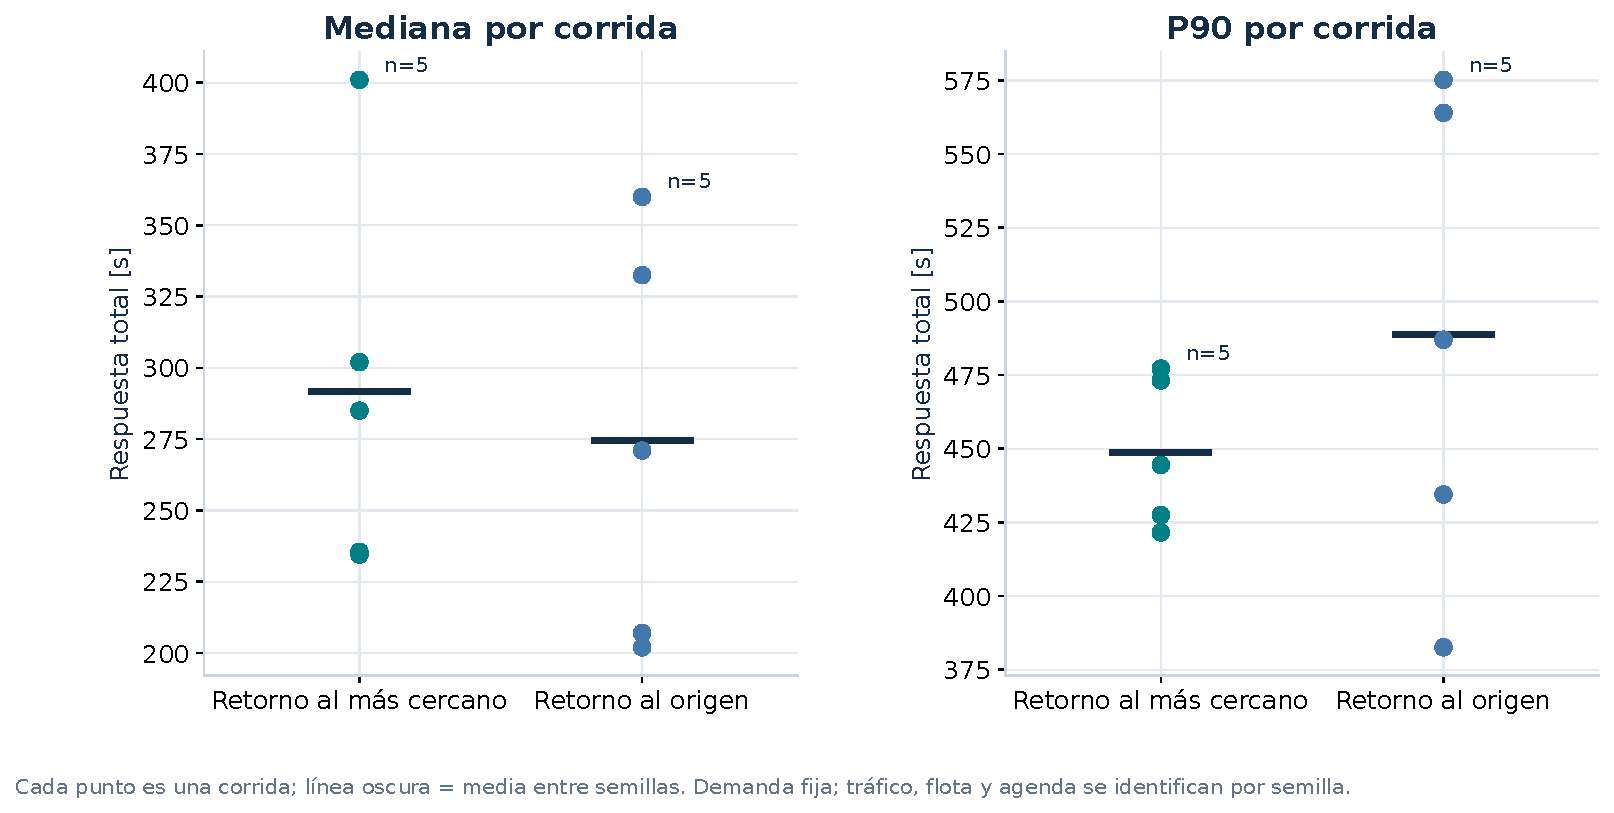
\includegraphics[width=0.95\textwidth]{07_extension.pdf}
\caption{Mediana y percentil 90 de cada réplica. La línea oscura representa la media entre semillas; los puntos conservan la variación observada.}
\label{fig:extension}
\end{figure*}

Con quince intentos por hora se observaron \EstresAcc{} accidentes y se cerraron \EstresCerr{} misiones. La mediana fue \EstresMed{} s y el percentil 90, \EstresP{} s. La espera de despacho siguió en cero. En esta ejecución no apareció saturación por falta de unidades; aumentar la agenda también cambió los lugares y la secuencia de choques, por lo que la mediana no creció de forma monótona. Todas las corridas comparadas terminaron sin tráfico pendiente.

La semilla 7 con retorno al origen se interrumpió a los 7.815 s por una aserción interna de \archivo{MSVehicle::getBackPositionOnLane} en SUMO 1.12.0. Sus resultados incompletos se excluyeron. Se eligió la semilla 8 para ambas políticas antes de observar sus resultados y se conservaron el log y los parámetros del fallo en \archivo{salida/fallos/origen_s7_t5/}.

\section{Validación y evidencia visual}
La auditoría ejecutó \Controles{} controles y no encontró errores de invariantes. Emitió \Advertencias{} advertencias, entre ellas la distancia hospitalaria, la ausencia de stock cero en una semilla distinta de la principal y los casos abiertos de la prueba negativa. Repetir la semilla 42 produjo \Repetidos{} archivos idénticos por SHA-256. Cinco pruebas adicionales aceptan la corrida válida y detectan un inventario alterado, tiempos modificados y un choque sin soporte XML; la prueba de negativa total verifica reintentos cada 30 s y conservación de unidades.

La validación A exige preparar red, tráfico, hospitales y flota. A1, A2 y A4 tienen evidencia técnica; A3 queda parcial por Patamarca. La validación B verifica los incidentes físicos, la elección de hospital, el retorno y los resultados. En la corrida principal se observaron \Accidentes{} choques dentro del rango $15\pm2$, en aristas distintas, con cero teletransportaciones, \Negativas{} negativas aleatorias y retornos que modifican el stock.

La demostración gráfica usa el mismo controlador. La Fig.~\ref{fig:guihospitales} conserva los siete puntos hospitalarios. En la Fig.~\ref{fig:guicola}, \GuiAcc{} presenta bus y moto inmóviles y tráfico detenido detrás, a los \GuiTiempo{} s. La Fig.~\ref{fig:guiretorno} corresponde al retorno de \GuiUnidad{} desde \GuiOrigen{} hacia \GuiDestino{}; el stock receptor aumentó de \GuiAntes{} a \GuiDespues{} a los \GuiRetorno{} s. Los estados se contrastan con los registros de TraCI. Las capturas apoyan la presentación ante el docente; esa evaluación aún debe realizarse.

\begin{figure*}[!t]
\centering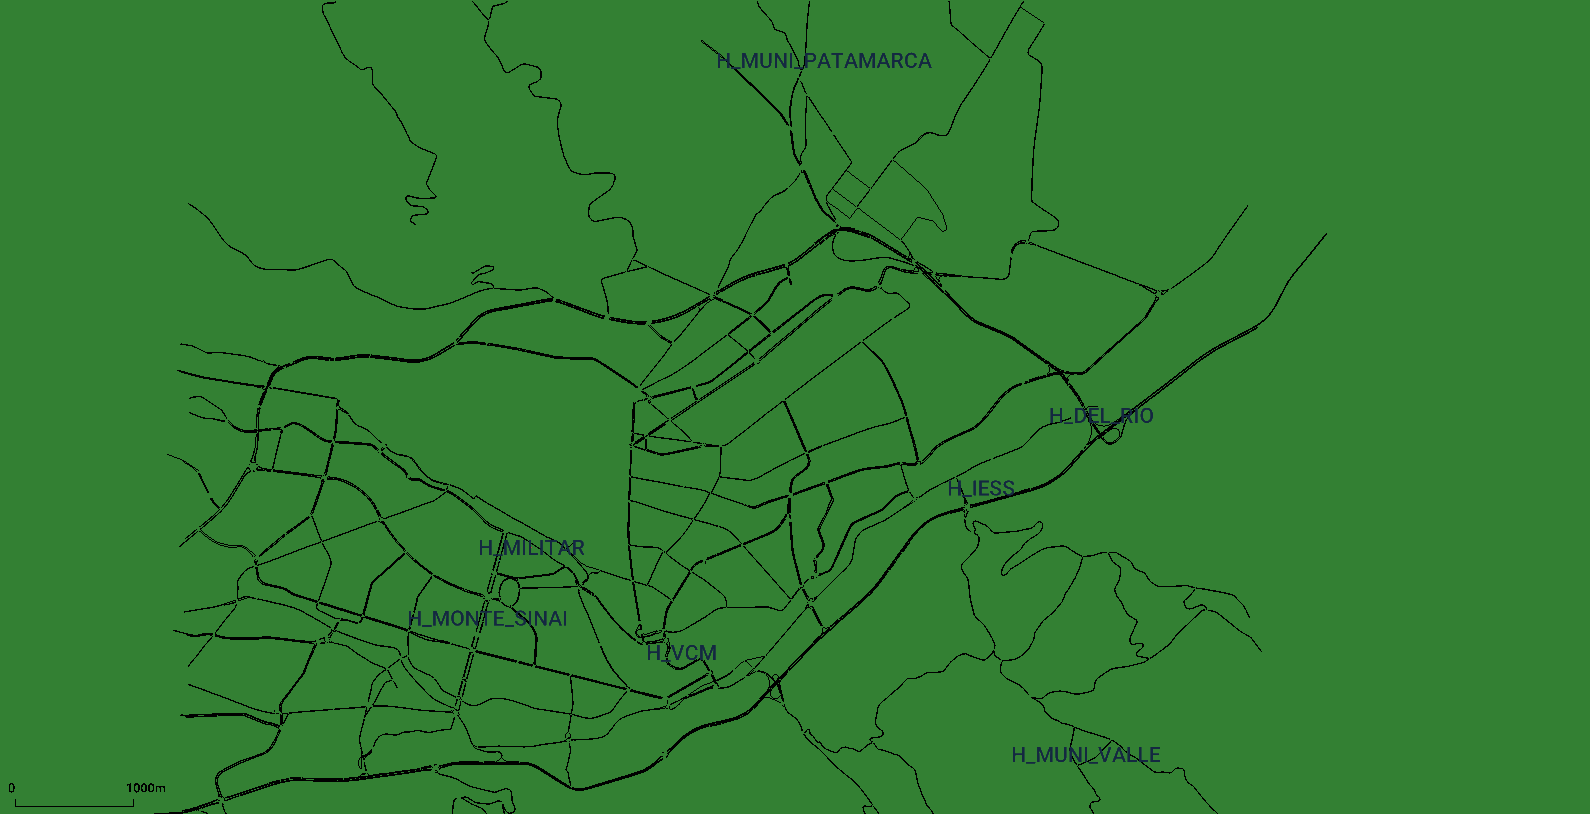
\includegraphics[width=0.95\textwidth]{01_hospitales.png}
\caption{Captura de SUMO-GUI con los siete hospitales. La demostración conserva también el inventario inicial en su registro estructurado.}
\label{fig:guihospitales}
\end{figure*}
\begin{figure*}[!t]
\centering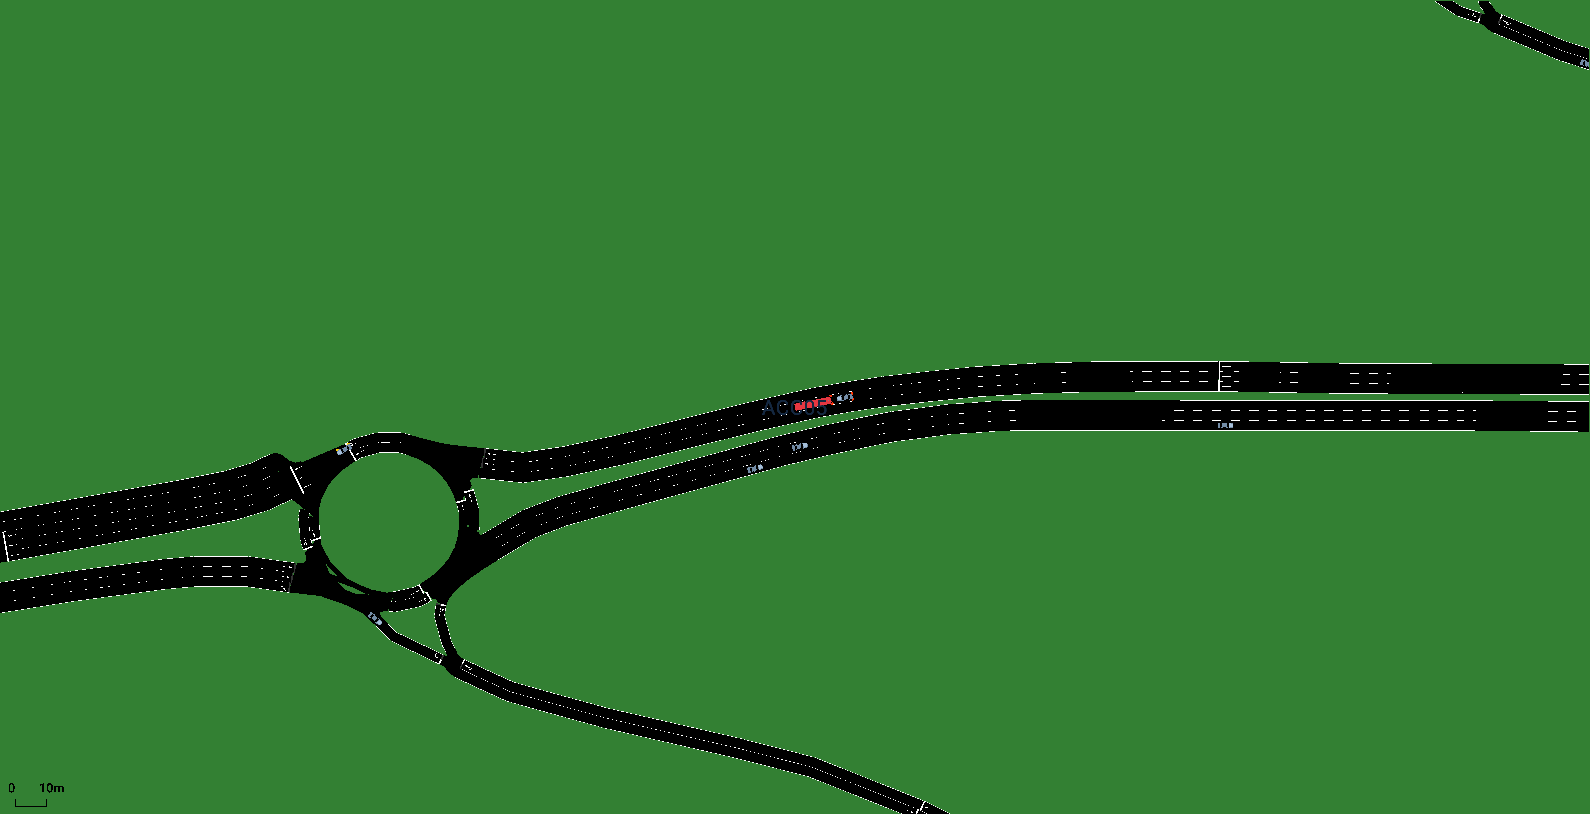
\includegraphics[width=0.95\textwidth]{02_accidente_cola.png}
\caption{Accidente físico con bus y moto en rojo y un vehículo de fondo detenido detrás. Estado registrado a los \GuiTiempo{} s.}
\label{fig:guicola}
\end{figure*}
\begin{figure*}[!t]
\centering
\includegraphics[width=0.95\textwidth]{03_retorno.png}
\caption{Hospital receptor después del retorno. La unidad ya se incorporó a su cola y dejó de circular; el aumento de stock de \GuiAntes{} a \GuiDespues{} consta en el log del mismo instante.}
\label{fig:guiretorno}
\end{figure*}

\section{Discusión y limitaciones}
La asignación de ambulancias depende de rutas dirigidas y disponibilidad. El ejemplo de despacho muestra por qué la distancia visual entre hospital y accidente resulta insuficiente para explicar la elección. El retorno cambia las bases desde las que podrán atenderse los siguientes incidentes; incluso un hospital inicialmente vacío puede participar después de recibir unidades.

Los tiempos obtenidos describen este escenario y sus parámetros. La flota no representa una medición del sistema sanitario de Cuenca. Los puntos hospitalarios son aproximaciones geométricas y el acceso de Patamarca supera el umbral solicitado. El criterio de atención a pie y la eliminación de vehículos por colisiones de fondo también influyen en la respuesta. Estos supuestos deben revisarse antes de interpretar la simulación como una estimación operativa.

La comparación utiliza cinco pares de semillas con demanda fija. Como las decisiones de retorno cambian el tráfico, los incidentes no son réplicas idénticas entre políticas. La diferencia media observada permite describir el experimento, pero no establece una ventaja universal. El fallo interno de una semilla confirma además la necesidad de conservar versión del simulador y registros de ejecución.

\section{Conclusiones}
El controlador completó las \Cerrados{} misiones de la corrida principal, conservó las diez ambulancias y terminó con la red vacía. La respuesta tuvo una mediana de \Mediana{} s y un percentil 90 de \Pnoventa{} s. La repetición exacta y la auditoría respaldan la consistencia de los registros de colisión, despacho y retorno.

El retorno cercano redistribuyó unidades y obtuvo una mediana menor en \ParesGana{} de cinco comparaciones. La carga de quince accidentes por hora completó todas sus misiones sin espera de despacho. Queda pendiente resolver el acceso hospitalario de Patamarca con una coordenada verificada para cumplir A3. La presentación de las validaciones A y B ante el docente completa la revisión de la práctica.

\appendices
\section{Reproducción y archivos de entrega}
El código, los datos, los archivos CSV/XML y las figuras están organizados en el proyecto \archivo{RetoAmbulancia}. \archivo{docs/COMANDOS.md} desarrolla todos los pasos; \archivo{docs/METODOLOGIA.md} explica las decisiones y \archivo{docs/DATOS.md} define las columnas. Desde la raíz, con Docker y la imagen \archivo{van3twin:jammy}, se ejecuta:
\begin{lstlisting}[language=bash]
python3 -m venv .venv
.venv/bin/python -m pip install -r requirements.txt
make reproducir PYTHON=.venv/bin/python
python3 scripts/comprobar_repeticion.py
python3 -m unittest discover -s pruebas -v
\end{lstlisting}
La demostración interactiva se inicia con \archivo{./scripts/demo_gui.sh}. El visor VNC se conecta a \archivo{localhost:5902}; la terminal se detiene para revisar hospitales, cola y retorno. Para regenerar capturas sin pausas se usa \archivo{make gui-validar}. La auditoría y el informe se actualizan con \archivo{make validar informe}.

El PDF usa la clase \archivo{IEEEtran} en modo conferencia, con dos columnas y referencias numeradas, de acuerdo con las herramientas de autor de IEEE\cite{ieee}. La fuente está en \archivo{docs/latex/Informe_Reto_Ambulancias.tex}; los valores y tablas se generan desde las salidas. Tectonic compila el documento y deja el registro en \archivo{docs/latex/build/}. Los archivos para publicación y el estado de entrega se describen en \archivo{docs/ENTREGA.md}.

El código, las capturas de SUMO-GUI y los resultados de esta práctica se reúnen en el repositorio público del autor:
\begin{center}
\href{https://github.com/angelrampolo/practica04-ambulancias-cuenca}{\nolinkurl{github.com/angelrampolo/practica04-ambulancias-cuenca}}
\end{center}
El archivo \archivo{README.md} describe la instalación y \archivo{docs/COMANDOS.md} detalla los comandos para reproducir cada fase.

\begin{thebibliography}{6}
\bibitem{guia} Universidad de Cuenca, ``Reto de accidentes bus-moto y despacho de ambulancias en Cuenca'', guía docente de Redes Vehiculares y Heterogéneas, archivo \archivo{Reto_Ambulancias_Docente_RVH.pdf}, 30 láminas, s. f.
\bibitem{osm} OpenStreetMap contributors, ``Copyright and License''. [En línea]. Disponible: \url{https://www.openstreetmap.org/copyright}. Consulta: 26 de octubre de 2026.
\bibitem{traci} Eclipse SUMO, ``Change Vehicle State'', documentación TraCI. [En línea]. Disponible: \url{https://sumo.dlr.de/docs/TraCI/Change_Vehicle_State.html}. Consulta: 26 de octubre de 2026.
\bibitem{routing} Eclipse SUMO, ``Routing''. [En línea]. Disponible: \url{https://sumo.dlr.de/docs/Simulation/Routing.html}. Consulta: 26 de octubre de 2026.
\bibitem{macro} Eclipse SUMO, ``Lane- or Edge-based Traffic Measures''. [En línea]. Disponible: \url{https://sumo.dlr.de/docs/Simulation/Output/Lane-_or_Edge-based_Traffic_Measures.html}. Consulta: 26 de octubre de 2026.
\bibitem{ieee} IEEE Author Center, ``Authoring Tools and Templates''. [En línea]. Disponible: \url{https://conferences.ieeeauthorcenter.ieee.org/write-your-paper/authoring-tools-and-templates/}. Consulta: 26 de octubre de 2026.
\end{thebibliography}
\end{document}
